Una entidad aprende si mejora su desempeño en tareas futuras en base a lo experimentado en el pasado. El aprendizaje puede variar desde lo simple, como lo exhibido al reconocer que ciertos objetos son peligrosos, hasta lo profundo, como lo exhibido al reflexionar sobre la mismísima existencia. En este capítulo hablaremos sobre una clase particular de aprendizaje, denominada como \ac{AS}, que si bien puede parecer a simple vista limitada, en realidad tiene amplia aplicabilidad: \emph{a partir de un conjunto de pares entrada-salida, aprender una función que infiera la salida para nuevas entradas}.

Más precisamente, este capítulo tiene como objetivo el de servir como una introducción al \ac{AS}. Introduciremos  el concepto de clasificación, presentaremos los modelos más populares utilizadas para llevarla a cabo, y describiremos cómo se lleva a cabo la evaluación en este tipo de tarea.
Por este motivo, los lectores ya familiarizados con la temática pueden pasarlo por alto y continuar su lectura directamente a partir del siguiente capítulo.

\section{Clasificación}
\label{sec:clasificacion}

Como se describe al inicio de la Sección 18.2 del conocido libro ``Artificial Intelligence: A Modern Approach'' de Stuart Russell y Peter Norving\cite{RussNorv10}, el \ac{AS} puede definirse más formalmente del siguiente modo:

\begin{quote}
    Dado un \textbf{conjunto de entrenamiento} con $N$ ejemplos de pares $(entrada,salida)$:
    $$(\pmb{x}_1,y_1),(\pmb{x}_2,y_2),\dots(\pmb{x}_N,y_N),$$
    donde cada $y_i$ fue generado por una función desconocida $y=\mathcal{F}(\pmb{x})$,\
    
    encontrar una función $h$ que aproxime la función desconocida $\mathcal{F}$.
\end{quote}

En este contexto, el aprendizaje puede verse como una búsqueda sobre el espacio de posibles funciones $h$ por una que se desempeñe bien, incluso con nuevas entradas más allá de las presentes en este conjunto de entrenamiento.
% Así, para medir el desempeño de una posible función $h$, es una práctica común el utilizar un \textbf{conjunto de prueba} con ejemplos que son distintos a los presentes en el conjunto de entrenamiento.
De hecho, se dice que la función $h$ \emph{generaliza bien} si predice correctamente los valores de $y$ para ejemplos nuevos, nunca antes vistos.

En la práctica, cada instancia de entrada $\pmb{x}$ estará normalmente representada por un vector de $m$ atributos, $\pmb{x}=\langle x_1,x_2,\dots,x_m\rangle$.
Tanto $\pmb{x}$ como $y$ podrían tener cualquier valor, no necesariamente numérico, sin embargo, cuando $y$ toma un valor de entre un conjunto finito de valores, al problema de aprendizaje supervisado se lo denomina como \textbf{clasificación} ---\emph{i.e.}, cuando $y\in C$ siendo $C=\{c_i,c_2,\dots,c_k\}$ y $k$ un entero positivo.
De este modo, cuando se trabaja con un problema de clasificación, a cada elemento $c_i$ del conjunto $C$ se lo denomina como ``clase'', ``categoría'' o simplemente ``etiqueta''.\footnote{En la práctica estas clases no serán más que simples etiquetas simbólicas, como ser ``spam'', ``no spam'', ``positivo'', ``negativo'', ``deportes'', ``tecnología'', etc.}
Así, un ejemplo de una tarea de clasificación sería, dado como entrada la reseña escrita por un usuario sobre un producto, predecir la etiqueta correcta de entre ``positiva'', ``negativa'' o ``neutra''.
Por lo tanto, y en resumen, dado una entrada $x$, clasificación es la tarea de predecir la etiqueta correcta para dicha entrada, habiendo previamente aprendido a realizar dicha tarea en base a un conjunto de entradas previamente etiquetadas, denominado como \textbf{conjunto de entrenamiento}.

Finalmente, en el problema de clasificación, es muy común referirse a la función $h$ que usamos para aproximar la función desconocida $\mathcal{F}$ como \textbf{modelo de clasificación} o simplemente como \textbf{clasificador}. En la siguiente sección se introducirán los clasificadores más conocidos.

\section{Modelos de Aprendizaje Automático para Clasificación}

Existe una gran variedad de modelos de aprendizaje automático que pueden ser empleados como clasificadores, en esta sección se describen brevemente los más ampliamente utilizados.

\subsection{Máquinas de Vectores Soporte}

\begin{figure}[t]
    \begin{subfigure}{0.5\textwidth}
        \centering
        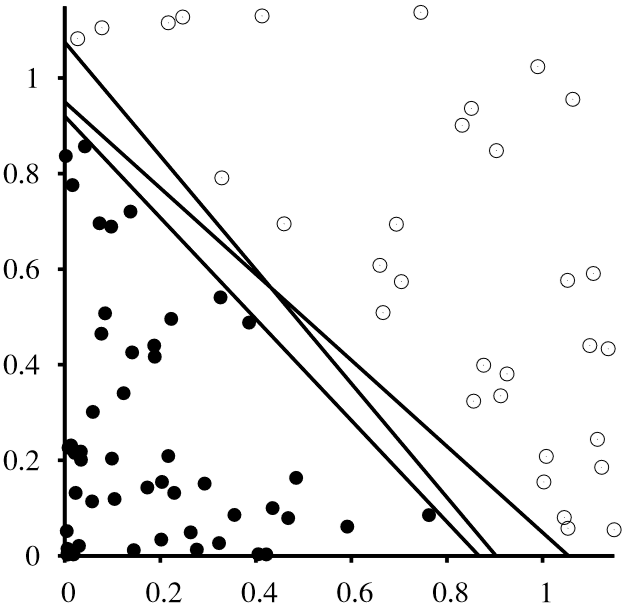
\includegraphics[width=\textwidth]{images/svm0}
        \caption{}
        \label{fig:svm_a}
    \end{subfigure}
    \begin{subfigure}{0.5\textwidth}
        \centering
        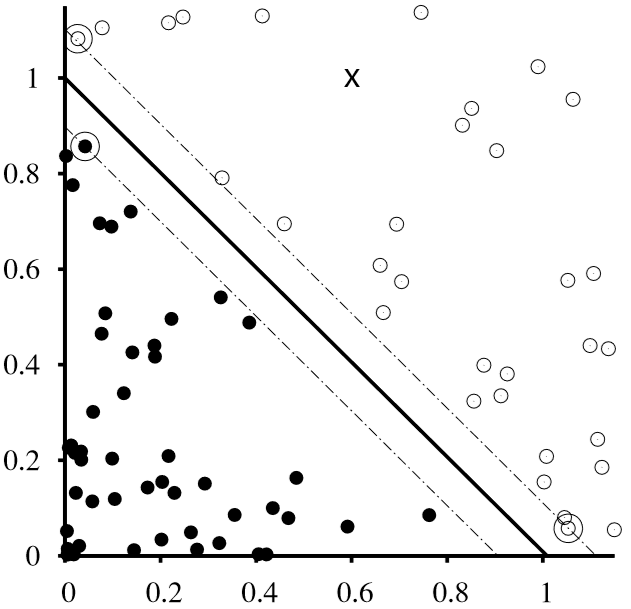
\includegraphics[width=\textwidth]{images/svm1}
        \caption{}
        \label{fig:svm_b}
    \end{subfigure}
\caption{
    Ejemplo sencillo de entrenamiento y clasificación con máquina de vectores soporte con dos clases, blanco y negro.
    (a) Instancias de entrenamiento etiquetadas (puntos blancos y negros) con tres separadores lineales candidatos de ejemplo.
    (b) Separador óptimo con máximo margen (linea sólida) encontrado luego del entrenamiento, el cual está justo en el punto medio del margen entre las dos clases (área entre las lineas puntadas).
    Los \emph{vectores soporte} de dicho separador son señalados con círculos grandes.
    Luego en (a), durante la clasificación, la nueva instancia $\langle 0.6, 1\rangle$ es ingresada (cruz negra), clasificándose como ``blanca'' por ubicarse por encima del separador, en la zona asociada a dicha clase.
}
\label{fig:svm}
\end{figure}

Desarrollado en AT\&T Bell Laboratories por Vapnik \emph{et al.}\cite{boser1992training,guyon1993automatic,cortes1995support,drucker1997support}, la Máquina de Vectores Soporte, o más popularmente conocida por su nombre en inglés como \ac{SVM}, es uno de los mejores, e incluso muchos creen que es el mejor, algoritmo de aprendizaje supervisado ``que viene listo para ser usado'': si uno no tiene ningún conocimiento previo especializado sobre un dominio, \ac{SVM} suele ser un excelente método para probar primero\cite{hsu2003practical}.

De forma abstracta, \ac{SVM} ve a cada instancia $\pmb{x}=\langle x_1,x_2,\dots,x_m\rangle$ como un punto en un espacio $m$-dimensional. Luego, durante el entrenamiento, utiliza todas las instancias de entrenamiento para encontrar el hiperplano óptimo que mejor divida las clases en ese espacio $m$-dimensional, es decir, el que tenga el máximo margen entre las dos clases.\footnote{\ac{SVM}, al ser un clasificador lineal, en principio sólo puede trabajar con dos clases. Sin embargo, esto no es una limitante ya que para trabajar con un número $k$ de clases mayor a 2, simplemente se utilizan $k$ modelos \ac{SVM} distintos, uno por cada clase.}
Así, al finalizar el entrenamiento, se tiene un hiperplano óptimo que divide el espacio $m$-dimensional en dos zonas, una asociada a cada clase. Finalmente, la clasificación se lleva a cabo simplemente viendo en cuales de esas dos zonas se ubica la instancia de entrada, $\pmb{x}$, al proyectarse en ese espacio $m$-dimensional.
Una característica particular de \ac{SVM} es que la solución al problema de clasificación está representada simplemente por los denominados como ``vectores soporte'', que no son otra cosa que las instancias de entrenamiento\footnote{Recordemos que cada instancia está representada como un vector de $m$ atributos, $\pmb{x}=\langle x_1,x_2,\dots,x_m\rangle$, de allí el nombre \emph{vectores} soporte.} más cercanas al separador óptimo.
Por ejemplo, suponiendo que nuestras instancias tuvieran sólo dos atributos, esto es $\pmb{x}=\langle x_1,x_2\rangle$, y pertenecieran a alguna de dos clases, digamos ``blanco'' o ``negro'', la \autoref{fig:svm} ilustra un posible ejemplo de entrenamiento, con el ``hiperplano óptimo'' (o en este caso ``línea óptima'') y sus respectivos vectores soporte, y un ejemplo de clasificación para una nueva instancia de entrada, $\langle 0.6, 1\rangle$.

\ac{SVM} también se pueden utilizar para problemas de clasificación no linealmente separables. En tales casos se utiliza lo que se conoce generalmente como el ``truco del kernel''\cite{scholkopf2001kernel}, en donde, haciendo uso de una función denominada como ``kernel'', las instancias son proyectadas a un nuevo espacio, de mayor dimensión, en donde las clases sí son  linealmente separables.


\subsection{Clasificadores Bayesianos Naïve}
\label{sec:mnb}

Los clasificadores bayesianos son una familia de clasificadores estadísticos que se basan en el teorema de Bayes, los cuales pueden predecir la probabilidad de pertenencia de una instancia dada a cada una de las clases\cite{murphy2006naive, rish2001empirical}. Más precisamente, dada una instancia de entrada a ser clasificada, la cual nuevamente está representada por un vector de $m$ atributos, $\pmb{x}=\langle x_1,x_2,\dots,x_m\rangle$, un clasificador bayesiano es un modelo capaz de calcular la probabilidad condicional, $P(c|\pmb{x})$, para cada una de las posibles clases $c$, clasificando finalmente a $\pmb{x}$ con la clase $c$ más probable de todas. Dado que, a diferencia de $P(c|\pmb{x})$, $P(\pmb{x}|c)$ puede aproximarse de forma directa utilizando todas las instancias $\pmb{x}$ disponibles en el conjunto de entrenamiento, la probabilidad condicional $P(c|\pmb{x})$ se calcula en base a $P(\pmb{x}|c)$ utilizando el teorema de Bayes del siguiente modo:

$$P(c|\pmb{x})=\frac{P(c)P(\pmb{x}|c)}{P(\pmb{x})}$$

Sin embargo, como para clasificar sólo es necesario encontrar la clase más probable, siendo $P(\pmb{x})$ independiente de cualquier clase $c$ y, por lo tanto, constante, para clasificar se prescinde del denominador, llevando a:

\begin{equation}
P(c|\pmb{x})\propto P(c)P(\pmb{x}|c)
\label{eq:mnb0}
\end{equation}


Los tipos de clasificadores bayesianos más ampliamente utilizados son los llamados como ``clasificadores bayesianos naïve'', los cuales suponen \emph{ingenuamente}\footnote{De allí que se utilice el término ``naïve''.} que, dada una categoría $c$, cada atributo $x_i$ de $\pmb{x}$ es condicionalmente independiente de todos los demás atributos $x_j$, con $i\ne j$.
Esta suposición se llama independencia condicional de clase\cite{lewis1998naive} y se utiliza con el fin de simplificar el cálculo de la clasificación, ya que al aplicarla se cumple que:

\begin{equation}
P(\pmb{x}|c)=P(x_1,x_2,\dots,x_m|c) = P(x_1|c)P(x_2|c)\dots P(x_m|c)
\label{eq:mnb1}
\end{equation}

Lo que permite, reemplazando \autoref{eq:mnb1} en \autoref{eq:mnb0}, realizar el cálculo involucrado simplemente en términos del producto de las probabilidades condicionales individuales de cada atributo, tal que así:

$$P(c|\pmb{x}) \propto P(c)P(x_1|c)P(x_2|c)\dots P(x_m|c) = P(c)\displaystyle\prod_{i=1}^{m}P(x_i|c)$$

Por lo que, finalmente, un clasificador bayesiano naïve clasificará a una instancia de entrada $\pmb{x}=\langle x_1,x_2,\dots,x_m\rangle$ calculando dicho producto para todas las clases y  seleccionado la que produzca el mayor resultado. En símbolos, siendo $C$ el conjunto de todas las clases, el clasificador seleccionará la clase $\hat{c}$ tal que:

\begin{equation}
\hat{c}=\argmax_{c\in C} P(c)\displaystyle\prod_{i=1}^{m}P(x_i|c)
\label{eq:mnb-prod}
\end{equation}

Sin embargo, una dificultad fundamental al realizar matemáticas continuas en una computadora digital es la necesidad de representar infinitos números reales con un número finito de bits. Esto significa que para casi todos los números reales se incurrirá en algún error de aproximación cuando sean representados en la computadora.\footnote{Típicamente utilizando números de puntos flotantes.} Una forma de error de redondeo, que es particularmente devastadora, es el \emph{underflow}, el cual ocurre cuando los números cercanos a cero se redondean a cero.
Por ese motivo, el cómputo de la \autoref{eq:mnb-prod} en la práctica falla convergiendo rápidamente a cero, ya que se trata de productos sucesivos de probabilidades (números reales pequeños positivos menores a uno). 
% Desde un punto de vista computacional, debido a la limitada precisión que las computadoras poseen para representar a los números reales utilizando sólo un número finito de bits,\footnote{Típicamente utilizando números de puntos flotantes.} el cómputo de productos sucesivos de números reales positivos menores a $1$ converge rápidamente a $0$.
Afortunadamente, cuando sólo interesa encontrar un valor máximo, como en esta ecuación, este problema normalmente se evita aplicando el logaritmo sobre la secuencia de productos, que de este modo se transforma en una secuencia de sumas.\footnote{Notar que al ser el logaritmo una función monótona creciente, este cambio no altera el resultado final de la ecuación, $\hat{c}$.}
Como consecuencia, los clasificadores bayesianos naïve en la práctica clasifican las instancias de entrada utilizando, en lugar de la \autoref{eq:mnb-prod}, la siguiente ecuación:

% $\log{\Big(P(c)\displaystyle\prod_{i=1}^{m}P(x_i|c)\Big)}$

\begin{equation}
\hat{c}=\argmax_{c\in C} \log{P(c)}+\sum_{i=1}^{m}\log{P(x_i|c)}
\label{eq:mnb-log}
\end{equation}

Finalmente, dependiendo de la tarea a abordar y la distribución de probabilidad que se asuma, será el clasificador en concreto con el que se trabaje y la manera concreta de calcular/aproximar las probabilidades.
Así, si se asume una distribución multinomial, el clasificador en concreto es denominado como ``clasificador bayesiano naïve multinomial'', o más popularmente conocido por su nombre en inglés como clasificador \ac{MNB}.
Por ejemplo, cuando se utiliza \ac{MNB} para abordar tareas de clasificación de texto, cada atributo $x_i$ suele corresponderse con una palabra $w_i$ del vocabulario aprendido, en cuyo caso las probabilidades de la \autoref{eq:mnb-log}, en la práctica, suelen calcularse utilizando la frecuencia de las palabras (estimación por máxima verosimilitud) del siguiente modo:

$$\hat{P}(w_i|c) = \frac{fr_{w_i,c}}{\sum_{w\in V}fr_{w,c}}$$

$$\hat{P}(c) = \frac{N_c}{N}$$

Donde $fr_{w_i,c}$ denota la frecuencia de la palabra $w_i$ en la clase $c$,\footnote{O la frecuencia más uno, en el caso de que se utilice un suavizado Laplace para evitar probabilidades igual a 0 para palabras desconocidas.} $V$ el vocabulario formado por todas las palabras presentes en el conjunto de entrenamiento, $N$ el número total de documentos en el conjunto de entrenamiento, y $N_c$ el número de documentos pertenecientes a la clase $c$. 
El clasificador \ac{MNB} es prácticamente el clasificador bayesiano por antonomasia en tareas de clasificación de texto, ya que al hacer corresponder cada atributo $x_i$ con cada palabra $w_i$, cada cual ocurriendo con una probabilidad $P(w_i|c)$, cada instancia $\pmb{x}=\langle x_1,x_2,\dots,x_m\rangle$ puede verse como una muestra generadas por, o tomada desde, una multinomial $(P(w_1|c),P(w_2|c),\dots,P(w_m|c))$.



\subsection{Redes Neuronales}

\begin{figure}[t]
    \centering
    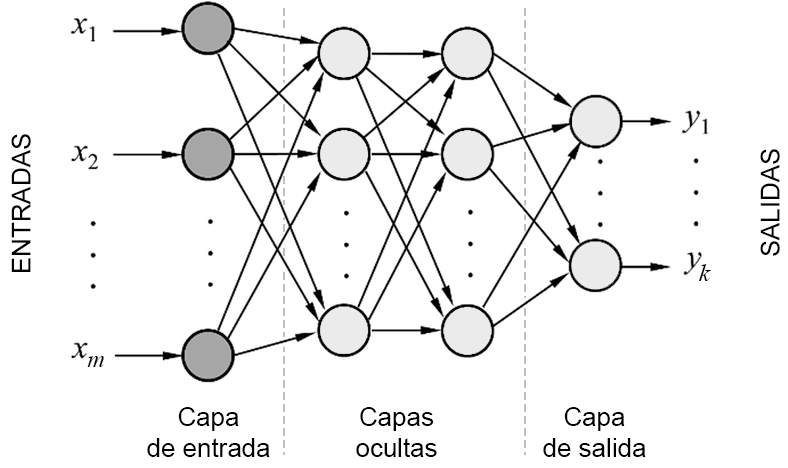
\includegraphics[width=120mm]{images/nn}
    \caption{Ejemplo de red neuronal de $m$ entradas y $k$ salidas. La red está compuesta por una capa de entrada con $m$ nodos de entradas, dos capas ocultas, y una capa de salida con $k$ nodos de salidas.}
    \label{fig:nn}
\end{figure}

Las redes neuronales artificiales, en inglés, \ac{ANN}, son modelos computacionales inspirados en el cerebro humano. Se denominan neuronales porque sus orígenes se encuentran en la ``neurona McCulloch-Pitts'' \cite{mcculloch1943logical}, un modelo simplificado de la neurona humana como una especie de elemento de cómputo que podría describirse en términos de lógica proposicional. Una \ac{ANN} es, en esencia, una red de pequeñas unidades de cómputo denominados como ``nodos'', ``neuronas'' o simplemente ``unidades'', las cuales típicamente se agrupan en distintos niveles, denominados como ``capas''\cite{basheer2000artificial,goodfellow2016deep}. Como se ilustra en la \autoref{fig:nn}, las redes neuronales tiene tres tipos de capas, a saber, de entrada, ocultas y de salida: la capa de entrada está compuesta por todos los nodos que reciben la entrada propiamente dicha, y cuya función es simplemente la de propagar la entrada hacia los nodos internos, sin modificarla; la capa de salida está compuesta por todos los nodos que generan la salida de la red, propiamente dicha; y finalmente, todas las otras capas, entre la entrada y la salida, son denominadas como capas ocultas.

\begin{figure}[t]
    \centering
    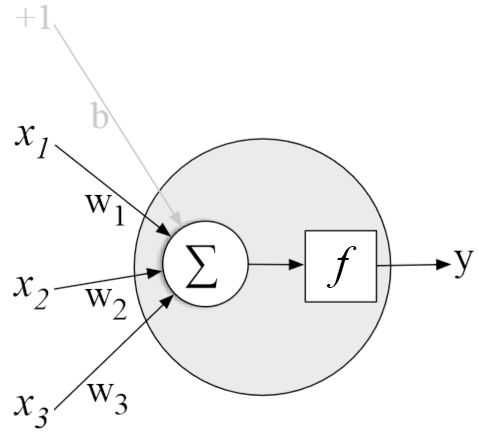
\includegraphics[width=60mm]{images/nn-node}
    \caption{Ejemplo de nodo con 3 entradas, $x_1$, $x_2$ y $x_3$.}
    \label{images/nn-node}
\end{figure}

Como se ilustra en la \autoref{images/nn-node}, cada nodo de una red neuronal toma un vector de valores de entrada, $\langle x_0,x_1,\dots,x_m\rangle$, y produce un único valor de salida, $y$, aplicando una función $f$ al producto punto entre el vector de entrada y un vector de pesos, $\langle w_0,w_1,\dots,w_m\rangle$, que cada nodo tiene asociado. Más precisamente, y en símbolos, la salida $y$ de un nodo se obtiene por:

$$y =  f\left(b + \sum_{i=0}^m w_i x_i\right)$$

La función $f$ se denomina como ``función de activación'' y su rol es determinar si el resultado del producto punto es suficiente como para que dicho nodo ``se active'' o no, esto es, si se propaga un valor de salida positivo ($y>0$) hacia los siguientes nodos o, de lo contrario, no se propaga ningún valor ($y=0$).\footnote{Algunas funciones de activación, como ser $\tanh$, pueden producir valores negativos ($y\leq0$).}
Tres de las funciones de activaciones más utilizadas son la función $softmax$, $tanh$, y $ReLu$\cite{ramachandran2017searching}.

El entrenamiento consiste en encontrar los valores adecuados para los pesos asociados a todos los nodos de la red. Existen distintos métodos para encontrar dichos valores, siendo ``backpropagation''\cite{chauvin1995backpropagation} el algoritmo más ampliamente utilizado actualmente. 
Cuando una \ac{ANN} es utilizada como un clasificador, habrá una nodo de entrada por cada atributo $x_i$ de la instancia de entrada, $\pmb{x}=\langle x_1,x_2,\dots,x_m\rangle$, y un nodo de salida por cada clase de interés. La clasificación se lleva a cabo alimentando a la red con la instancia de entrada, $\pmb{x}$, y asignando la etiqueta asociada al nodo de salida que produce el mayor valor.

\

En la actualidad, con el aumento del poder de cómputo basado en el uso de GPU y la masiva disponibilidad de datos, las redes neuronales normalmente llegan a ser considerablemente profundas, con un gran número de capas ocultas y miles de nodos, lo que permite que se desempeñen asombrosamente bien en una gran variedad de tareas, como ser en el reconocimiento de voz y en el reconocimiento de imágenes. Esto produjo una gran proliferación de distintas arquitecturas de redes profundas, denominadas como ``arquitecturas de aprendizaje profundo''\cite{goodfellow2016deep}. %, tales como redes neuronales recurrentes, redes neuronales convoluciones o redes de creencias profundas.

\subsection{K Vecinos Más Próximos}

El \ac{ABI} es una familia de algoritmos de aprendizaje que, en lugar de realizar una generalización explícita, compara las nuevas instancias de entrada directamente con las instancias disponibles en el conjunto de entrenamiento.
Esto es, en lugar de llevar a cabo una fase de entrenamiento para construir una abstracción con las instancias de entrenamiento, en \ac{ABI} se representa cada instancia de entrada $\pmb{x}$ como un punto en un espacio $m$-dimensional ---en otras palabras, cada instancia es representada por un vector de $m$ atributos, $\pmb{x}=\langle x_1,x_2,\dots,x_m\rangle$. Luego, las nuevas instancias de entradas serán clasificadas directamente en base a las etiquetas que tienen asignadas las instancias de entrenamiento más cercanas, en ese espacio $m$-dimensional.

La idea principal detrás de estos algoritmos es que instancias similares deben pertenecer a categorías similares, es decir, la etiqueta para la entrada debería ser la misma que tienen las instancias cercanas. El concepto de ``cercanía'' implícitamente conlleva la necesidad de definir formalmente el concepto de ``similitud'' entre pares de instancias. Para ello, es necesario utilizar una \emph{función de similitud} que calcula la distancia entre instancias. Además, los modelos basados en \ac{ABI} también tienen que definir una función, o política de clasificación, que especifique cómo se clasificará efectivamente la entrada en base a las etiquetas de las instancias cercanas.

Existen varios clasificadores basados en \ac{ABI} tales como el ``k Vecinos Más Próximos'' y el algoritmo K*, entre otros\cite{witten2002data}. De entre estos, el más ampliamente utilizado es el primero, ``k Vecinos Más Próximos'', que es más conocido por su nombre en inglés como \ac{k-NN}.

\ac{k-NN} se basa en el algoritmo ``Vecino Más Próximo''\cite{cover1967nearest}, el cual usando alguna función de distancia dada\cite{prasatha2017effects},\footnote{Típicamente distancia coseno, euclidiana, o Manhattan.} determina cuál de todas las instancias del conjunto de entrenamiento es la más similar a la instancia dada, clasificando a esta última con la misma etiqueta que tiene asignada esta instancia más cercana.
\ac{k-NN} generaliza este algoritmo, encontrando no sólo la instancia más cercana, sino las $k$ instancias más cercanas a la nueva, clasificándola, finalmente, en base a la etiqueta que predomina entre todas ellas\cite{zhang2017efficient}.


\subsection{Árboles de Decisión}


\begin{figure}
    \centering
    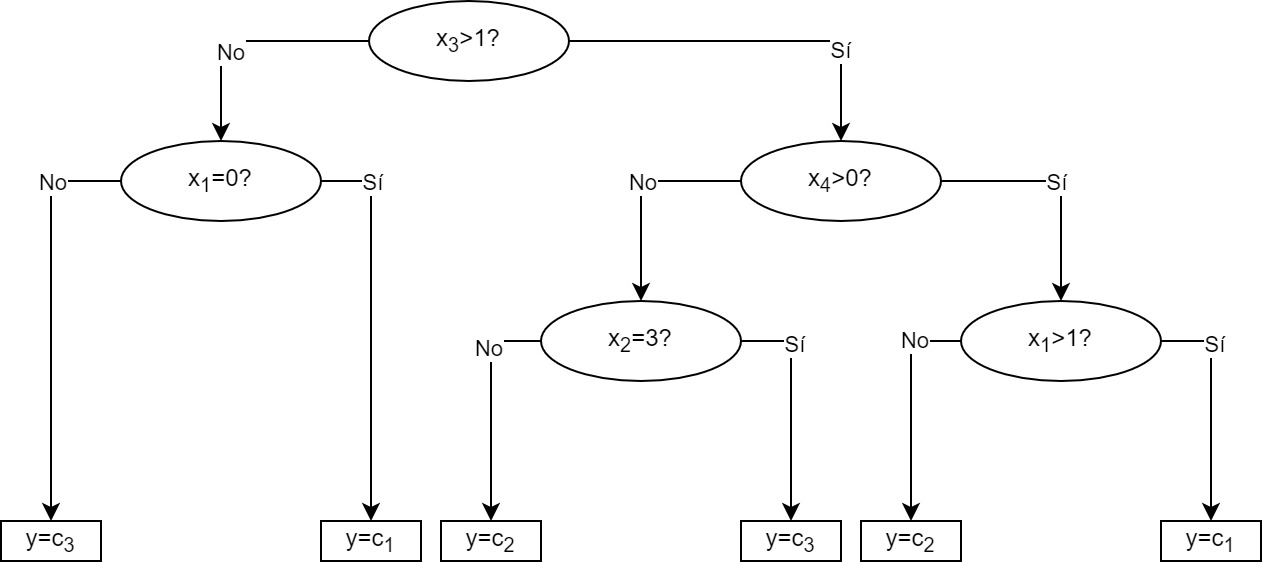
\includegraphics[width=\textwidth]{images/dt}
    \caption{Ejemplo sencillo de un árbol de decisión.}
    \label{fig:ad}
\end{figure}


Los \ac{AD} fueron aplicados por primera vez al modelado del lenguaje por Bahl \emph{et al.} para estimar la probabilidad de las palabras habladas\cite{bahl1989tree}.
Un árbol de decisión es una representación gráfica en la que cada nodo interno está asociado a una decisión sobre uno de los atributos que conforman la entrada, y los nodos terminales (hojas) están asociados con una etiqueta de clase.
Más en concreto, cada nodo interno está normalmente asociado a una condición lógica, la cual puede ser verdadera o falsa, sobre un atributo en particular de la entrada\cite{breslow1997simplifying}.%, que a su vez se enlaza con nuevos nodos en relación a cada posible respuesta a dicha decisión.
Por ejemplo, suponiendo que la entrada está conformada por 4 atributos, en símbolos, $\pmb{x}=\langle x_1,x_2,x_3,x_4\rangle$, y la salida $y$ puede tomar valores de etiqueta, $y\in\{c_1,c_2,c_3\}$, entonces un ejemplo de árbol de decisión podría ser el mostrado en \autoref{fig:ad}.

La construcción de los \ac{AD} generalmente implica un proceso recursivo de división del conjunto de entrenamiento para elegir el atributo de cada nodo interno. Así, se comienza seleccionando el atributo más relevante/discriminativo para todo el conjunto de entrenamiento como raíz del árbol.
Luego se crea un nuevo subárbol hijo por cada posible respuesta a la condición lógica de este nodo raíz. Finalmente, cada subárbol se construye recursivamente siguiendo este mismo proceso, usando sólo un subconjunto del conjunto de entrenamiento, obtenido al dividirlo según la condición lógica asociada a dicho subárbol.
Uno de los principales problemas a la hora de construir un árbol de decisiones es determinar qué atributo debe elegirse como ``el más relevante''. Un atributo relevante debe poder dividir, tanto como sea posible, las instancias de entrenamiento entre las diferentes clases.
Para llevar a cabo esto, en la práctica se utilizan medidas provenientes de la Teoría de la Información\cite{shannon1948mathematical}, como la entropía, la entropía relativa, la complejidad de Kolmogorov, entre otras\cite{chandola2009anomaly}.

Los \ac{AD} representan el ``estándar de oro'' de los modelos basados en el paradigma ``divide y vencerás''. Sin embargo, el tamaño, la complejidad y la dispersión de datos suelen conducir a clasificaciones erróneas cuando los árboles se vuelven lo suficientemente grandes.



\section{Evaluación de Clasificadores}

Una vez seleccionado el modelo de clasificación a utilizar, y de entrenarlo con los datos disponibles en el conjunto de entrenamiento, es necesario poder saber si realmente el modelo funciona, es decir ¿es posible confiar en sus predicciones? ¿Podría el modelo simplemente haber memorizado los datos con los que se lo entrenó y, por lo tanto, en la práctica no desempeñarse adecuadamente con nuevas instancias?
La capacidad de un modelo de clasificar correctamente nuevas instancias desconocidas se denomina como \emph{capacidad de generalización}\cite{schmidhuber1997discovering,xu2017information}.
Así, en el aprendizaje automático, es crucial poder evaluar cada modelo para poder cuantificar qué tan buena es su capacidad de generalización en el problema en particular que está siendo abordado.
Evaluar el modelo con los datos utilizados para el entrenamiento no es aceptable, ya que puede generar fácilmente modelos sobreoptimistas y sobreajustados, por lo que la evaluación siempre debe utilizar un conjunto de instancias nunca antes vistas.
Existen dos métodos para llevar esto a cabo como parte del proceso de desarrollo del modelo, ``retención'' y ``validación cruzada''.
El primer método consiste en dividir aleatoriamente el conjunto de datos etiquetados completo en tres subconjuntos, denominados como ``entrenamiento'', ``validación'' y ``prueba'', utilizando sólo el primero para entrenar y reteniendo los últimos dos para utilizarlos del siguiente modo:

\begin{itemize}
    \item \textbf{Conjunto de validación}: se utiliza para ajustar y evaluar el rendimiento del modelo durante la fase de entrenamiento. Es decir, proporciona una plataforma de prueba para ajustar los hiperparámetros del modelo, permitiendo seleccionar los mejores posibles.\footnote{Por lo tanto, los modelos sin parámetros pueden prescindir de este conjunto de validación.}
    \item \textbf{Conjunto de prueba}: como está formado por instancias nunca vistas y que, a diferencia del anterior, no interfieren en el entrenamiento, este conjunto se utiliza para evaluar efectivamente el (probable) rendimiento futuro del modelo. Por ejemplo, si el modelo se desempeña mucho mejor con el conjunto de validación que con este conjunto, el modelo no generaliza bien y probablemente la causa sea que la combinación de hiperparámetros seleccionada estén sobreajustados a los datos de entrenamiento.
\end{itemize}

Finalmente, el método ``validación cruzada'' también implica dividir el conjunto de datos etiquetados completo en subconjuntos, pero esta división forma parte de un proceso iterativo. El modelo se entrena y se evalúa con distintos subconjuntos complementarios en cada iteración y, una vez finalizado el proceso, los resultados obtenidos en cada iteración se promedian para dar una estimación del rendimiento general del modelo\cite{seni2010ensemble}.

La técnica de validación cruzada más común es la llamada ``validación cruzada de $k$ iteraciones'', en donde el conjunto de datos original se divide en $k$ subconjuntos de igual tamaño, denominados como ``pliegos''. El valor de $k$ es especificado por el usuario, siendo 3, 4, 5 o 10 los más usados, típicamente dependiendo del tamaño total del conjunto de datos.
Luego, en cada una de las $k$ iteraciones, se selecciona un nuevo pliego para ser utilizado como conjunto de prueba,\footnote{O validación, dependiendo de si se haya reservado un conjunto aparte para ser usado como conjunto de prueba luego de la validación cruzada o no.} y el conjunto de entrenamiento se forma juntando los $k-1$ pliegos restantes.
La ``validación cruzada de $k$ iteraciones'' es una técnica extremadamente popular debido a su robustez, ya que cada instancia de dato llega a estar en un conjunto de prueba exactamente una vez, y llega a estar en un conjunto de entrenamiento $k-1$ veces. Esto reduce significativamente el riesgo de sesgo y sobreajuste, debido a que se utilizan la mayoría de los datos tanto para entrenar como para probar el modelo. 

\

Hasta aquí hemos hablado sobre los métodos para evaluar los modelos dentro del proceso de desarrollo de los mismos, pero no se ha hablado sobre cómo se mide efectivamente su desempeño.
En la siguiente subsección se describen brevemente las medidas de evaluación más ampliamente utilizadas para llevar a cabo dicha tarea.


\subsection{Medidas de Desempeño}
\label{sec:medidas}

Una medida de desempeño cuantifica el rendimiento de un modelo predictivo e implica comparar la etiqueta de clase esperada con la etiqueta de clase predicha.
Existen una gran variedad de métricas estándares que se utilizan ampliamente para evaluar modelos de clasificación\cite{ferri2009experimental}, diseñadas para obtener la fracción, la proporción o la tasa con la que la clase predicha no coincide con la esperada en un conjunto de datos de prueba/evaluación.

Quizás una de las métricas más utilizada es el ``accuracy'', la cual nos indica la proporción de instancias que fueron correctamente clasificadas, esto es:

\begin{equation}
accuracy = \frac{clasificaciones\ correctas}{clasificaciones\ totales}
\label{eq:accuracy}
\end{equation}

El \emph{accuracy} parece lo bastante adecuado, sencillo e intuitivo como para ser usado en cualquier problema a abordar. Sin embargo, esta medida no hace distinciones entre clases, es decir, las respuestas correctas se tratan por igual independientemente de la clase. A veces esto no es adecuado ya que es posible que se desee conocer cuántas instancias fallaron en cada clase. Éste sería el caso si el costo de una clasificación errónea varía según la clase o si se tienen muchos más datos de prueba para una clase que para otra. Por ejemplo, clasificar a un usuario de Twitter como ``depresivo'' cuando no lo es (falso positivo) tiene consecuencias muy distintas a clasificarlo como ``no depresivo'' cuando en realidad sí lo es (falso negativo).

Es por este motivo que muchas veces una manera mucho más adecuada de evaluar el desempeño de un clasificador es utilizando la denominada ``matriz de confusión'', cuya idea general es contar el número de veces que las instancias de cierta clase se clasifican como otra o no.\footnote{Es por esto que se denomina ``matriz de confusión'', ya que hace que sea fácil ver si el clasificador \emph{confunde} las clases, etiquetando incorrectamente con frecuencia a una como otra.}

Más precisamente, una matriz de confusión es una tabla en la que cada fila se corresponde con una clase y contiene el número de instancias predichas para esa clase, desagregadas, a su vez, en columnas, según la clase real de dichas instancias\cite{powers2011evaluation}.
Esto permite visualizar rápidamente el número total de falsos positivos, falsos negativos, verdaderos positivos y verdaderos negativos. Por ejemplo, la siguiente tabla muestra dónde se ubicarían estos valores en una matriz de confusión de $2\times2$ para dos clases hipotéticas, ``Positivo'' y ``Negativo'':

\

\begin{tabular}{l l|c|c|c}
\multicolumn{2}{c}{}&\multicolumn{2}{c}{Realidad}&\\
% \cline{3-4}
\multicolumn{2}{c|}{} & Positivo & Negativo\\
\cline{2-4}
\multirow{2}{*}{Predicción}& Positivo & \begin{tabular}{@{}c@{}}Número de \\ Verdaderos Positivos \\ (\#VP)\end{tabular} &  \begin{tabular}{@{}c@{}}Número de \\ Falsos Positivos \\ (\#FP)\end{tabular} \\
\cline{2-4}
& Negativo & \begin{tabular}{@{}c@{}}Número de \\ Falsos Negativos \\ (\#FN)\end{tabular} & \begin{tabular}{@{}c@{}}Número de \\ Verdaderos Negativos \\ (\#VN)\end{tabular}\\
\cline{2-4}
\end{tabular}

\

La matriz de confusión habilita un análisis más detallado que la mera proporción de clasificaciones correctas dada por el \emph{accuracy}, ya que,  además, brinda información sobre qué clases se predicen correctamente, cuáles incorrectamente y qué tipo de errores se están cometiendo.
Sin embargo, en lugar de utilizar la matriz de confusión completa, a menudo es conveniente utilizar medidas de desempeño que capturen, y resuman en un único valor, cierta información específica presente en la matriz que sea de especial interés para el problema abordado.
Dentro de estas medidas, las más ampliamente conocidas y utilizadas son ``precision'', ``recall'', y ``$F_\beta$''. La primera responde a la pregunta ``de las instancias que el clasificador predijo como de cierta clase, ¿cuántas realmente lo fueron?''; la segunda responde a ``de todas las instancias que pertenecen a cierta clase, ¿cuántos fueron efectivamente clasificadas como tal?''; mientras que la tercera simplemente combina estas dos primeras en una sola, intentando equilibrar ambos aspectos.

Más precisamente, la \emph{precision}, a veces denotada por $\pi$\cite{sebastiani2002machine}, puede interpretarse como la probabilidad de que una predicción positiva\footnote{Por ``positiva'', ``positivo'' o ``clase positiva'' entenderemos aquí, y hasta el final del capítulo, como la clase de nuestro interés, es decir, aquella que estemos interesados en medir.} realmente lo sea. Esta métrica nos sintetiza el porcentaje de instancias clasificadas como positivas que efectivamente lo fueron, en fórmula:

\begin{equation}
precision = \frac{\#VP}{\#VP + \#FP}
\label{eq:precision}
\end{equation}


De igual modo, el \emph{recall}, a veces denotada por $\rho$\cite{sebastiani2002machine}, sintetiza el porcentaje de todas las instancias positivas que fueron, efectivamente, clasificadas correctamente, calculándose como:

\begin{equation}
recall = \frac{\#VP}{\#VP + \#FN}
\label{eq:recall}
\end{equation}

Finalmente, como se mencionó anteriormente, la medida $F_\beta$ busca combinar \emph{precision} y \emph{recall} a través de una media armónica que mide la efectividad de la clasificación teniendo en cuenta que se le da, proporcional a $\beta$, una importancia  mayor al \emph{recall} que a la \emph{precision}. Más precisamente, y en símbolos, se tiene que:

\begin{equation}
F_\beta = (1 + \beta^2) \times \frac{precision\times recall}{\beta^2 \times precision + recall}
\label{eq:fbeta}
\end{equation}


Dado que $\beta=1$ indicaría que se da igual importancia tanto a \emph{recall} como a \emph{precision}, $F_1$ es con frecuencia la medida $F$ más ampliamente utilizada:

\begin{equation}
F_1 = 2 \times \frac{precision\times recall}{precision + recall}
\label{eq:f1}
\end{equation}

Notar que el valor $F_1$ será pequeño si alguno de los dos, \emph{precision} o \emph{recall}, lo son, ya que, a diferencia de la media aritmética, la media armónica tiende hacia el menor de los valores ---por lo tanto, su valor se maximiza sólo cuando los valores están ``en armonía'', \emph{i.e.} cuando ambos valores son cercanos entre sí.
\hfill$\square$
